% Six short algebraic notes from Grothendieck's working notes (folders 2, 22, 46, 77, 153, 158) — standalone article for Hexagon.
% pdfLaTeX. Compile: latexmk -pdf article.tex (or tectonic -X compile article.tex).
\documentclass[11pt,a4paper]{amsart}
\usepackage[T1]{fontenc}
\usepackage[utf8]{inputenc}
\usepackage{lmodern,microtype,amssymb,mathtools,enumitem}
\usepackage[margin=2.7cm]{geometry}
\usepackage{tikz}
\usepackage[hidelinks]{hyperref}
\usepackage{xurl}
\emergencystretch=3em

\newtheorem{theorem}{Theorem}[section]
\newtheorem{proposition}[theorem]{Proposition}
\newtheorem{lemma}[theorem]{Lemma}
\newtheorem{corollary}[theorem]{Corollary}
\theoremstyle{definition}
\newtheorem{definition}[theorem]{Definition}
\theoremstyle{remark}
\newtheorem{remark}[theorem]{Remark}
\newtheorem{example}[theorem]{Example}

\newcommand{\Z}{\mathbb Z}
\newcommand{\Q}{\mathbb Q}
\newcommand{\F}{\mathbb F}
\newcommand{\cO}{\mathcal O}
\newcommand{\fac}[1]{\href{https://grothendieck.umontpellier.fr/#1.pdf}{folder~#1}}

\title[Six short algebraic notes]{Six short algebraic notes,\\ after Grothendieck's working notes}
\author{Michel Hua}
\address{Commutator, Paris, France}
\email{michel@commutator.io}
\thanks{ORCID 0009-0002-8304-0683.}
\date{7 November 2026}
\subjclass[2020]{13-02; 19L10, 13J05, 20J06, 13F20, 11E08, 18A30}
\keywords{Chern classes, lambda-rings, formal smoothness, non-abelian cohomology, integer-valued polynomials, discriminant of quadratic forms, cofiltered categories, Lean}

\begin{document}
\begin{abstract}
Six independent results from Grothendieck's working notes, each a few pages long in the original, are stated and proved here, completed or corrected where the pages are incomplete.
(1) For $K = \Z[L]/(L-1)^n$, the comparison map from the ring generated by Chern classes to the graded ring of the $\gamma$-filtration is surjective but not injective as soon as $n \ge 3$, the kernel being killed by $(n-1)!$.
(2) If $\Omega_{K/k}$ is infinite-dimensional, $K[[t_1, \dots, t_n]]$ is not formally smooth over $K$ for the discrete topology: no derivation extends $d_K$.
(3) A $1$-cocycle of a finite group with values in the units of a finite algebra over a local ring, trivial modulo the maximal ideal, is trivial when the order of the group is invertible; there are Sylow and tame-inertia versions.
(4) The co-operations on relative integer-valued polynomials are well defined under a flatness condition.
(5) For the universal quadratic form of even rank $2n$, $(-1)^n\det$ of its polar matrix is a square modulo $4$, the square of a sum over perfect matchings.
(6) A finite, non-empty, connected category in which every connected presheaf has a simply connected category of elements is cofiltered; for monoids, the pages' Proposition~1.
All results are formalised in Lean.
\end{abstract}

\maketitle

\section*{Introduction}

The University of Montpellier holds the mathematical papers that Alexandre Grothendieck left to Jean Malgoire, and publishes their facsimiles. Besides long programmes, they contain short computations that settle, or try to settle, one precise question. This paper collects six of them, from \fac{2}, \fac{22}, \fac{46}, \fac{153}, \fac{77} and \fac{158}, one section each; the sections can be read independently. Statements are attributed to Grothendieck when the page states them, with the page; otherwise they are said to be \emph{after} the page, and the change is described. The proofs are ours unless we say that we follow the page. Every result is formalised in Lean~4 with Mathlib (Section~\ref{sec:lean}).

\section{A Chern ring that is not the graded \texorpdfstring{$\gamma$}{gamma}-ring}\label{sec:chern}

Folder~2, on the Riemann--Roch theorem, keeps integral Chern classes. Page~21 attaches two rings to a $\lambda$-ring $K$ with ``geometric'' elements \cite{fultonlang1985}: the \emph{Chern ring} $CK$, generated by symbols $c^i(x)$ subject to the Whitney formula, the product rule and $c^i(E) = 0$ above the rank of a geometric $E$; and the graded ring $GK$ of the $\gamma$-filtration. A map $\varphi_K\colon CK \to GK$ sends $c^i(x)$ to the class of $\gamma^i(x - \varepsilon(x))$. The page asks whether $\varphi_K$ is injective.

\begin{lemma}[Grothendieck, \fac{2}, p.~9]\label{lem:point}
For $r \ge 1$ and any commutative ring $A$, in $A[\eta]/(\eta^{r+1})$:
\[
\prod_{i=0}^{r}(1 - i\eta)^{(-1)^i\binom ri} = 1 + (-1)^{r-1}(r-1)!\,\eta^r.
\]
\end{lemma}

This is the total Chern class of a point, computed through a Koszul resolution; the factor $(r-1)!$ is the price of integral coefficients. Take $K = \Z[L]/(L - 1)^n$, the $K$-ring of $\mathbb P^{n-1}$ with only $L$ declared geometric. Then $CK$ is generated by $\zeta = c^1(L)$; with $\xi = 1 - L^{-1}$, the only relation is $c(\xi^n) = 1$, and Lemma~\ref{lem:point} gives $CK = \Z[\zeta]/I$, where $I$ is generated by the $a_m\zeta^m$, $a_m$ the coefficient of $\zeta^m$ in the product, while $GK = \Z[\zeta]/(\zeta^n)$.

\begin{theorem}[Grothendieck, \fac{2}, p.~21]\label{thm:chern}
For $n \ge 3$, $\zeta^n$ is non-zero in $CK$ and $(n-1)!\,\zeta^n = 0$; $GK$ is torsion-free, and $\varphi_K$ is surjective but not injective. For $n \le 2$, $\varphi_K$ is bijective.
\end{theorem}

\begin{proof}
The $a_m$ vanish for $1 \le m < n$ and $a_n = \pm(n-1)!$, so $I \subseteq (\zeta^n)$ and $(n-1)!\,\zeta^n = 0$. To see $\zeta^n \ne 0$, send $\zeta$ to $h$ in $T = (\Z/(n-1)!)[h]/(h^{n+1})$: the relations hold there, and $h^n \ne 0$ as soon as $(n-1)! > 1$, that is $n \ge 3$. For $n \le 2$, $a_n = \pm1$ and $I = (\zeta^n)$.
\end{proof}

The page affirms $\zeta^3 \ne 0$ for $n = 3$ without showing it; the map to $T$ does.

\section{Power series and the discrete topology}\label{sec:power}

Folder~22 gathers complements to EGA~$0_{\rm IV}$ (1963 to about 1967). Its typescript, numbered 24 to 32 in his hand, proves the noetherian case of Chase's theorem \cite{chase1960}: if every finitely generated $A$-module is finitely presented, every product of flat $A$-modules is flat, because $M \otimes_A \prod_i P_i \to \prod_i(M \otimes_A P_i)$ is an isomorphism for $M$ finitely presented. Handwritten pages~22--24 then ask whether $A = k[[t]]$, with the discrete topology, is formally smooth over $k$; page~22 presumes that it never is when $k = \Q(x_i)$ has infinitely many variables.

\begin{theorem}[Grothendieck, \fac{22}, p.~23]\label{thm:power}
Let $k$ be a commutative ring and $K$ a field that is a $k$-algebra with $\Omega_{K/k}$ of infinite dimension over $K$, and $A = K[[t_1, \dots, t_n]]$, $n \ge 1$. No derivation $D\colon A \to A \otimes_K \Omega_{K/k}$ satisfies $D(c) = 1 \otimes dc$ for $c \in K$. Hence $A$ is not formally smooth over $K$ for the discrete topology.
\end{theorem}

\begin{proof}[Sketch]
Choose $c_0, c_1, \dots \in K$ with $dc_0, dc_1, \dots$ linearly independent, and consider $f = \sum_j c_jt_1^j \in A$. A derivation $D$ extending $d$ would satisfy, for every $N$, $D(f) = \sum_{j<N}t_1^j \otimes dc_j + t_1^N D(g_N)$, where $f = \sum_{j<N} c_jt_1^j + t_1^Ng_N$; but an element of $A \otimes_K \Omega_{K/k}$ involves only finitely many independent differentials, while the $t_1^j$-coefficients of $D(f)$ must contain all the $dc_j$. Formal smoothness would give such a $D$ as a retraction of the first-order thickening.
\end{proof}

Pages~26 and~28 find that differentials need not inject in characteristic~$p$:

\begin{proposition}[Grothendieck, \fac{22}, pp.~26 and~28]\label{prop:diff}
Let $p$ be prime, $K = \F_p(x, b_0, \dots, b_{p-1})$, $a_i = b_i^p$, $y = \sum_{i<p} a_ix^i$, $k = \F_p(x, y) \subset K$ and $k' = k \cap K^p$. Then $K \otimes_k \Omega_{k/k'} \to \Omega_{K/k'}$ is not injective: $dy - y'\,dx$, with $y' = \sum_i ia_ix^{i-1}$, is a non-zero element of the kernel.
\end{proposition}

\section{Lifting cocycles through the reduction modulo \texorpdfstring{$\mathfrak m$}{m}}\label{sec:coh}

Folder~46 ends its ``petits fourbis cohomologiques'' (pages~71--92) with a semi-local Hilbert~90. Let $\cO$ be a commutative local ring with maximal ideal $\mathfrak m$ and residue field of characteristic~$p$, $\Gamma$ a finite group, and $A$ an $\cO$-algebra, not necessarily commutative, on which $\Gamma$ acts by ring automorphisms; the margin of page~90 cites $A = \mathrm M_n(\cO)$. A $1$-cocycle is $c\colon\Gamma \to A^*$ with $c(gh) = c(g)\,g(c(h))$, and $c$, $c'$ are cohomologous if $c(g) = u^{-1}c'(g)\,g(u)$ for some $u \in A^*$.

\begin{theorem}[after \fac{46}, pp.~90--92]\label{thm:lift}
Suppose $p \nmid |\Gamma|$, and $\mathfrak m^NA = 0$ for some $N$ or $A$ finite over $\cO$. Let $A \to B$ be a surjective $\Gamma$-compatible ring map with kernel in $\mathfrak mA$, for instance $B = A/\mathfrak mA$. Then $H^1(\Gamma, A^*) \to H^1(\Gamma, B^*)$ is injective: two cocycles with cohomologous reductions are cohomologous.
\end{theorem}

\begin{proof}
Elements $1 + x$, $x \in \mathfrak mA$, are units, by nilpotence or Nakayama, so an element of $A$ is a unit as soon as its image in $B$ is. Let $v \in B^*$ with $\bar c(g) = v^{-1}\bar c'(g)\,g(v)$, lift $v$ to $w \in A$, and put $u = \sum_{\sigma\in\Gamma} c'(\sigma)\,\sigma(w)\,c(\sigma)^{-1}$. The cocycle relations give $c'(g)\,g(u) = u\,c(g)$. In $B$, every term of the sum is $v$, so $u$ reduces to $|\Gamma|\,v$, a unit since $|\Gamma|$ is invertible in $\cO$. Hence $u \in A^*$ and $c(g) = u^{-1}c'(g)\,g(u)$.
\end{proof}

The page argues differently and states the result for $p \nmid |\Gamma|$ ``in particular'', after a Sylow version, which we prove in the following form.

\begin{theorem}[after \fac{46}, p.~90 and its margin]\label{thm:sylow}
Let $\Lambda \le \Gamma$ have index prime to $p$, for instance a $p$-Sylow subgroup, $A$ finite over $\cO$, and $A \to B$ as above with $A^\Lambda \to B$ surjective (implied by the margin's surjectivity of $A^\Gamma \to A/\mathfrak mA$). A class of $H^1(\Gamma, A^*)$ that is trivial in $H^1(\Gamma, B^*)$ and in $H^1(\Lambda, A^*)$ is trivial; if $A$ is commutative, $H^1(\Gamma, A^*) \to H^1(\Gamma, B^*) \times H^1(\Lambda, A^*)$ is injective.
\end{theorem}

\begin{proof}[Sketch]
Average over $\Gamma/\Lambda$ instead of $\Gamma$: with $c(\lambda) = u^{-1}\lambda(u)$ on $\Lambda$ and $w \in A^\Lambda$ lifting $\pi(u)\bar v^{-1}$, the element $z = u^{-1}w$ satisfies $c(\lambda)\lambda(z) = z$, so $b = \sum_{g\Lambda} c(g)\,g(z)$ is well defined, satisfies $c(\gamma)\gamma(b) = b$, and reduces to $[\Gamma:\Lambda]\,\bar v^{-1}$, a unit.
\end{proof}

Pages~84--89 treat a semi-local base on which $\Gamma$ acts, with decomposition and inertia groups $\Gamma_d \supseteq \Gamma_i$.

\begin{theorem}[after \fac{46}, pp.~84--89]\label{thm:inertia}
Let $\cO$ be a commutative local ring with infinite residue field $k$, $\Gamma$ a finite group acting on $\cO$ with inertia $\Gamma_i$ of order invertible in $k$, and $A$ a finite $\cO$-algebra with a semi-linear action of $\Gamma$. Then $H^1(\Gamma, A^*) \to H^1(\Gamma_i, A^*)$ is injective. In particular, if $\Gamma$ acts faithfully on $k$, $H^1(\Gamma, A^*) = 1$; for $\mathfrak m = 0$ this is Hilbert's Theorem~90 for any finite algebra over an infinite field.
\end{theorem}

\begin{proof}[Sketch]
Reduce to $c = c'$ on $\Gamma_i$ and work in $B = A/\mathfrak mA$ with the twisted semi-linear action $\gamma\star x = c'(\gamma)\gamma(x)c(\gamma)^{-1}$. A Speiser-type lemma, through Dedekind's independence of characters and $|\Gamma_i| \ne 0$ in $k$, shows that the $\Gamma_i$-fixed vector $1$ lies in the $k$-span of the fixed points $X$ of the twisted action. A determinant polynomial in the coordinates on $X$ takes the value $1$, hence does not vanish identically on $(k^\Gamma)^n$, since $k^\Gamma$ is infinite: some $k^\Gamma$-combination of fixed points is a unit. It makes $\bar c$ and $\bar c'$ cohomologous, and Theorem~\ref{thm:lift}'s averaging, with an element of trace one for $\Gamma_i$, lifts the coboundary to $A$.
\end{proof}

For the global semi-local statement (decomposition and inertia groups of a noetherian semi-local ring on whose maximal ideals $\Gamma$ acts transitively), see Lorenz \cite{lorenz1999} for related non-abelian $H^1$ computations; the full statement of pages~84--89 is not proved here.

\section{Co-operations on relative integer-valued polynomials}\label{sec:int}

Folder~153, \emph{Analyseurs}, looks for the abstract structure of a ring of operations with a composition, now called a plethory \cite{tallwraith1970, borgerwieland2005}, through integer-valued polynomials \cite{cahenchabert1997, elliott2010}. Page~3 fixes an inclusion of commutative rings $k_0 \subseteq K_0$ and
\[
\Omega = \{F \in K_0[T] \mid F(\lambda) \in k_0 \text{ for all } \lambda \in k_0\},
\]
and wants $F(X + Y)$ and $F(XY)$, for $F \in \Omega$, to be ``well-determined'' elements of $\Omega \otimes_{k_0} \Omega$. Let $\beta\colon K_0 \otimes_{k_0} \Omega \to K_0[T]$ be the multiplication map.

\begin{theorem}[after \fac{153}, pp.~3 and~9]\label{thm:int}
Let $K_0$ be any commutative $k_0$-algebra.
\begin{enumerate}
\item $\beta$ is surjective.
\item If $\beta$ is injective and $\Omega$ is free over $k_0$, then $\Omega \otimes_{k_0} \Omega \to K_0[X, Y]$ is injective, its image is the set of polynomials taking values in $k_0$ on $k_0 \times k_0$, and $F(X + Y)$, $F(XY)$ are images of unique elements of $\Omega \otimes_{k_0} \Omega$: $\Omega$ carries a co-addition and a co-multiplication.
\item $\beta$ is injective when $K_0$ is a localisation of $k_0$ and $\Omega$ is free, and when $K_0$ is flat over $k_0$ with $K_0 \otimes_{k_0} K_0 = K_0$.
\end{enumerate}
\end{theorem}

\begin{proof}[Sketch]
(1) The monomials $T^n$ lie in $\Omega$ and span $K_0[T]$ over $K_0$. (2) In a basis $(e_j)$ of $\Omega$, the $1 \otimes e_j$ form a basis of $K_0 \otimes \Omega$, and surjectivity and injectivity of $\beta$ say that the $e_j$ span $K_0[T]$ and are $K_0$-independent; the co-operations follow coordinate by coordinate. (3) In the flat case, $\beta$ is $\mathrm{id} \otimes (\Omega \hookrightarrow K_0[T])$, injective by flatness, followed by the multiplication $K_0 \otimes_{k_0} K_0[T] \to K_0[T]$, which is the multiplication of $K_0 \otimes_{k_0} K_0$ coefficient by coefficient.
\end{proof}

For $k_0 = \Z$, $K_0 = \Q$, $\Omega$ has the binomial basis $\binom Tn$ of page~2, and one recovers the classical biring structure of $\mathrm{Int}(\Z)$ \cite{elliott2010}.

\section{The universal discriminant modulo 4}\label{sec:disc}

Folder~77, part IV, takes the universal quadratic form $q = \sum_i Y_ix_i^2 + \sum_{i<j}Y_{ij}x_ix_j$ over $\Z[Y]$ in $m$ variables and the determinant of its polar matrix $P_m$, which has $2Y_i$ on the diagonal and $Y_{ij}$ off it. Page~68 shows $\det P_m \equiv 0 \bmod 2$ for $m$ odd, and for $m = 2n$ puts
\[
B_{2n} = \sum_M \prod_{\{i,j\} \in M} Y_{ij},
\]
the sum over perfect matchings $M$ of $\{1, \dots, 2n\}$ (the hafnian of the off-diagonal part), and looks for $\varepsilon = \pm1$ with $B_{2n}^2 - \varepsilon\det P_{2n} \equiv 0 \bmod 4$, ``predicting'' $\varepsilon = (-1)^n$.

\begin{theorem}[Grothendieck, \fac{77}, pp.~68--71]\label{thm:disc}
For every $n \ge 0$, $4$ divides $(-1)^n\det P_{2n} - B_{2n}^2$ in $\Z[Y]$. Hence there is $C_{2n} \in \Z[Y]$ with $(-1)^n\det P = B^2 - 4C$ for every quadratic form of rank $2n$ over every commutative ring. The other sign fails: for $n = 1$ and $n = 2$, $B^2 + (-1)^n\det P$ is not divisible by $4$ in general.
\end{theorem}

\begin{proof}
Expand $\det P = \sum_\sigma \operatorname{sgn}(\sigma)\prod_i P_{i\sigma(i)}$ and read each permutation as a graph on $\{1, \dots, 2n\}$: fixed points, transpositions (double edges) and cycles of length $\ge 3$. A fixed point contributes a factor $2Y_i$. For a permutation with $c$ cycles of length $\ge 3$, reversing any of these cycles gives $2^c$ permutations with the same sign and the same product. Modulo $4$, only two kinds of terms survive. (a) Fixed-point-free involutions, that is perfect matchings $M$, with sign $(-1)^n$ and product $\prod_{M}Y_{ij}^2$. (b) Permutations without fixed points having exactly one cycle of length $\ge 3$, which then has even length $2\ell$ since the rest consists of transpositions; they come in pairs and contribute $2\prod Y$ each pair, signs being irrelevant modulo $4$. (A permutation with one fixed point and only transpositions does not exist on an even set, and every other configuration carries a factor $4$.) On the other side, $B^2 = \sum_M \prod_M Y^2 + 2\sum_{\{M, M'\}}\prod_M Y\prod_{M'} Y$, and $M \cup M'$ is a union of double edges and alternating even cycles. Pairs whose union has $c \ge 2$ long cycles come in groups of $2^{c-1}$ with the same product, hence vanish modulo $4$; pairs with exactly one long cycle correspond bijectively to the pairs of terms (b), with the same product. So $(-1)^n\det P \equiv B^2 \bmod 4$. For the other sign: with $n = 1$, $a_1 = a_2 = 0$, $b_{12} = 1$, $B^2 - \det P = 2$; with $n = 2$ and $b_{12} = b_{34} = 1$, the rest zero, $B^2 + \det P = 2$.
\end{proof}

Figure~\ref{fig:match} shows the graphs for $n = 2$. In rank $2$, $-\det P = b_{12}^2 - 4a_1a_2$ is the usual discriminant; in rank~$4$ the edition writes $C_4$ explicitly, as page~87 checks the coefficients. The page's alarm in brown ink, corrected two lines below, concerned this comparison. The invariant is the classical discriminant of an even-rank quadratic form over a ring \cite{knus1991}; the hafnian description of its square root modulo~$4$ is what the pages add.

\begin{figure}[ht]
\centering
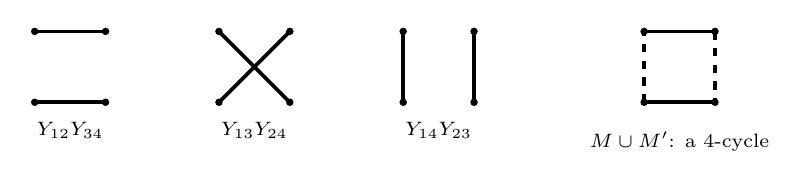
\begin{tikzpicture}[scale=0.9]
\foreach \dx/\a/\b/\c/\d in {0/1/2/3/4, 2.6/1/3/2/4, 5.2/1/4/2/3} {
  \begin{scope}[xshift=\dx cm]
  \foreach \k/\x/\y in {1/0/1, 2/1/1, 3/1/0, 4/0/0} { \coordinate (p\k) at (\x,\y); }
  \draw[line width=1.3pt] (p\a) -- (p\b); \draw[line width=1.3pt] (p\c) -- (p\d);
  \foreach \k in {1,2,3,4} { \fill (p\k) circle (1.5pt); }
  \node[font=\scriptsize] at (0.5,-0.4) {$Y_{\a\b}Y_{\c\d}$};
  \end{scope}
}
\begin{scope}[xshift=8.6cm]
  \foreach \k/\x/\y in {1/0/1, 2/1/1, 3/1/0, 4/0/0} { \coordinate (q\k) at (\x,\y); }
  \draw[line width=1.3pt] (q1) -- (q2); \draw[line width=1.3pt] (q3) -- (q4);
  \draw[line width=1.3pt, dashed] (q2) -- (q3); \draw[line width=1.3pt, dashed] (q4) -- (q1);
  \foreach \k in {1,2,3,4} { \fill (q\k) circle (1.5pt); }
  \node[font=\scriptsize, align=center] at (0.5,-0.55) {$M \cup M'$: a 4-cycle};
\end{scope}
\end{tikzpicture}
\caption{Rank $4$: the three perfect matchings of $\{1,2,3,4\}$, whose sum is $B_4$, and the union of two of them, an alternating $4$-cycle. Its two orientations are the two $4$-cycle terms of $\det P$; together they contribute $2\,Y_{12}Y_{23}Y_{34}Y_{41}$, the cross term of $B_4^2$ modulo $4$.}\label{fig:match}
\end{figure}

\section{Finite categories with simply connected elements}\label{sec:cof}

Folder~158, \emph{Autour des Dérivateurs}, dated about 1990--1991, studies one question: is a small category $X$ cofiltered as soon as condition (H) holds, that every connected presheaf on $X$ has a simply connected category of elements? Pages~44--53 treat finite categories, starting with monoids, categories with one object. A monoid $M$ is \emph{pseudo-cofiltered} if for all $u, v$ there are $u', v'$ with $uu' = vv'$, and \emph{cofiltered} if moreover for all $u, v$ there is $w$ with $uw = vw$.

\begin{theorem}[Grothendieck, \fac{158}, Proposition~1, pp.~44--46]\label{thm:monoid}
Let $M$ be a finite pseudo-cofiltered monoid whose enveloping group is trivial (every monoid map to a group is trivial). Then there is $p \in M$ with $up = p$ for all $u \in M$, and $M$ is cofiltered.
\end{theorem}

\begin{proof}[Sketch, following the page]
Realise $M$ as a monoid of maps of a set $E$ by right multiplication; finiteness makes a minimal non-empty image $E_0 = uE$ stable, and on $E_0$ the monoid acts by permutations (``comme $E_0$ est fini, on en conclut que $u(E_0) = E_0$''). The resulting map to a symmetric group is trivial by hypothesis, so $E_0$ is a single point $p$, fixed by every $u$. Then $uw = vw$ with $w = p$.
\end{proof}

\begin{theorem}[after \fac{158}, p.~52]\label{thm:cof}
In any small category, (H) implies that two elements of a connected presheaf have a common ancestor; in a non-empty connected category, two arrows $u\colon x \to c$, $v\colon y \to c$ complete to a square $uu' = vv'$. A finite, non-empty, connected category satisfying (H) is cofiltered. Connectedness is needed: the discrete category with two objects satisfies (H) and is not cofiltered.
\end{theorem}

For a monoid with a minimal element, the corollary of page~39 states that (H) implies cofiltered; conversely, for every cofiltered monoid, the category of elements of a connected $M$-set is simply connected. Whether (H) implies cofiltered for every small category, the question of the folder, is not settled here.

\section{Verification}\label{sec:lean}
\begingroup\sloppy
The statements proved above are formalised in Lean~4 with Mathlib, in the files \nolinkurl{Folder2.lean}, \nolinkurl{Folder22.lean}, \nolinkurl{Folder46.lean}, \nolinkurl{Folder153.lean}, \nolinkurl{Folder77.lean} and \nolinkurl{Folder158.lean} of the repository \href{https://github.com/Commutator-IO/grothendieck-project}{Commutator-IO/grothendieck-project} (directory \nolinkurl{lean/Grothendieck}), using only Lean's standard axioms. Not proved here: the geometric statement of folder~2, page~13, on an elliptic curve; the semi-local Hilbert~90 of folder~46 in full; the co-operations of folder~153 under the weaker hypothesis $K_0 \otimes K_0 = K_0$ alone; the question of folder~158 for infinite categories.
\endgroup

\section*{Statement on the use of artificial intelligence}
The transcriptions of the folders, the modernised readings, the proofs, the Lean formalisation and a first draft of this text were produced with language models (Claude Opus~5 and Opus~5.5, Anthropic), under the author's direction. The author checked the statements, the proofs and the references, and takes full responsibility for the content. The formal proofs are checked mechanically by Lean.

\section*{Acknowledgements}
The facsimiles are published by the University of Montpellier, \href{https://grothendieck.umontpellier.fr/}{grothendieck.umontpellier.fr}.

\begin{thebibliography}{9}
\bibitem{borgerwieland2005} J.~Borger, B.~Wieland, Plethystic algebra, \emph{Adv.\ Math.} 194 (2005), 246--283, \href{https://doi.org/10.1016/j.aim.2004.06.006}{doi:10.1016/j.aim.2004.06.006}.
\bibitem{cahenchabert1997} P.-J.~Cahen, J.-L.~Chabert, \emph{Integer-Valued Polynomials}, Math.\ Surveys Monogr.~48, Amer.\ Math.\ Soc., 1997, \href{https://doi.org/10.1090/surv/048}{doi:10.1090/surv/048}.
\bibitem{chase1960} S.~U.~Chase, Direct products of modules, \emph{Trans.\ Amer.\ Math.\ Soc.} 97 (1960), 457--473, \href{https://doi.org/10.1090/S0002-9947-1960-0120260-3}{doi:10.1090/S0002-9947-1960-0120260-3}.
\bibitem{elliott2010} J.~Elliott, Birings and plethories of integer-valued polynomials, \emph{Actes des rencontres du CIRM} 2 (2010), no.~2, 53--58, \href{https://doi.org/10.5802/acirm.34}{doi:10.5802/acirm.34}.
\bibitem{fultonlang1985} W.~Fulton, S.~Lang, \emph{Riemann--Roch Algebra}, Grundlehren der mathematischen Wissenschaften~277, Springer, 1985, \href{https://doi.org/10.1007/978-1-4757-1858-4}{doi:10.1007/978-1-4757-1858-4}.
\bibitem{knus1991} M.-A.~Knus, \emph{Quadratic and Hermitian Forms over Rings}, Grundlehren der mathematischen Wissenschaften~294, Springer, 1991, \href{https://doi.org/10.1007/978-3-642-75401-2}{doi:10.1007/978-3-642-75401-2}.
\bibitem{lorenz1999} M.~Lorenz, $K_0$ of invariant rings and nonabelian $H^1$, \emph{J.\ Algebra} 214 (1999), 458--478, \href{https://doi.org/10.1006/jabr.1998.7725}{doi:10.1006/jabr.1998.7725}.
\bibitem{tallwraith1970} D.~O.~Tall, G.~C.~Wraith, Representable functors and operations on rings, \emph{Proc.\ London Math.\ Soc.} (3) 20 (1970), 619--643, \href{https://doi.org/10.1112/plms/s3-20.4.619}{doi:10.1112/plms/s3-20.4.619}.
\end{thebibliography}

\end{document}
